\documentclass[tikz,border=2pt]{standalone}
\usepackage{amsmath}
\usetikzlibrary{arrows.meta}
\begin{document}
% Prisoner's Dilemma (payoffs = minus years in prison). Starting from (M,M) = (-2,-2), each player
% alone gains 1 by finking (-1 > -2 for player 1, -1 > -2 for player 2), but when both fink the result
% is the equilibrium (F,F) = (-4,-4), which leaves both 2 worse off than (M,M).
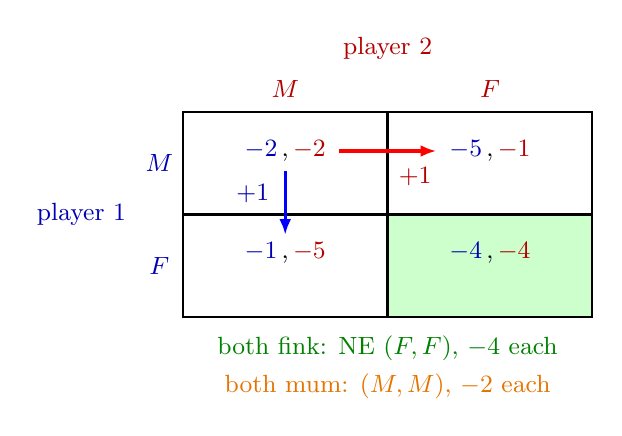
\begin{tikzpicture}[font=\small, >={Latex[length=2mm]}]
  \def\w{2.6} \def\h{1.3}
  % equilibrium cell
  \fill[green!20] (\w,-\h) rectangle (2*\w,0);
  \draw[thick] (0,-\h) rectangle (2*\w,\h);
  \draw[thick] (\w,-\h) -- (\w,\h);
  \draw[thick] (0,0) -- (2*\w,0);
  % strategy labels
  \node[red!70!black] at (0.5*\w,\h+0.3) {$M$};
  \node[red!70!black] at (1.5*\w,\h+0.3) {$F$};
  \node[blue!70!black] at (-0.3,0.5*\h) {$M$};
  \node[blue!70!black] at (-0.3,-0.5*\h) {$F$};
  \node[red!70!black, anchor=south] at (\w,\h+0.55) {player 2};
  \node[blue!70!black, anchor=east] at (-0.6,0) {player 1};
  % payoffs
  \node at (0.5*\w,0.62*\h) {\textcolor{blue!70!black}{$-2$}\,,\,\textcolor{red!70!black}{$-2$}};
  \node at (1.5*\w,0.62*\h) {\textcolor{blue!70!black}{$-5$}\,,\,\textcolor{red!70!black}{$-1$}};
  \node at (0.5*\w,-0.38*\h) {\textcolor{blue!70!black}{$-1$}\,,\,\textcolor{red!70!black}{$-5$}};
  \node at (1.5*\w,-0.38*\h) {\textcolor{blue!70!black}{$-4$}\,,\,\textcolor{red!70!black}{$-4$}};
  % unilateral temptations from (M,M)
  \draw[->, very thick, blue] (0.5*\w,0.42*\h) -- (0.5*\w,-0.2*\h);
  \node[blue!70!black, anchor=east] at (0.5*\w-0.08,0.2*\h) {$+1$};
  \draw[->, very thick, red] (0.5*\w+0.68,0.62*\h) -- (1.5*\w-0.68,0.62*\h);
  \node[red!70!black, anchor=north] at (\w+0.35,0.62*\h-0.08) {$+1$};
  % summary under the table
  \node[green!50!black, anchor=north] at (\w,-\h-0.12) {both fink: NE $(F,F)$, $-4$ each};
  \node[orange!90!black, anchor=north] at (\w,-\h-0.6) {both mum: $(M,M)$, $-2$ each};
\end{tikzpicture}
\end{document}
